\documentclass{article}

\usepackage{fancyhdr}
\usepackage{extramarks}
\usepackage{amsmath}
\usepackage{amsthm}
\usepackage{amsfonts}
\usepackage{tikz}
\usepackage[plain]{algorithm}
\usepackage{algpseudocode}
\usepackage{tikz,pgfplots,multicol}

\usetikzlibrary{automata,positioning}

%
% Basic Document Settings
%

\topmargin=-0.45in
\evensidemargin=0in
\oddsidemargin=0in
\textwidth=6.5in
\textheight=9.0in
\headsep=0.25in

\linespread{1.1}

\pagestyle{fancy}
\lhead{\hmwkAuthorName}
\chead{\hmwkClass\ (\hmwkClassInstructor\ \hmwkClassTime)}
\rhead{\hmwkTitle}
\lfoot{\lastxmark}
\cfoot{\thepage}

\renewcommand\headrulewidth{0.4pt}
\renewcommand\footrulewidth{0.4pt}

\setlength\parindent{0pt}

\setcounter{secnumdepth}{0}
\newcounter{partCounter}
\newcounter{homeworkProblemCounter}
\setcounter{homeworkProblemCounter}{1}
\nobreak\extramarks{Problem \arabic{homeworkProblemCounter}}{}\nobreak{}

%
% Homework Problem Environment
%
% This environment takes an optional argument. When given, it will adjust the
% problem counter. This is useful for when the problems given for your
% assignment aren't sequential. See the last 3 problems of this template for an
% example.
%
\newenvironment{homeworkProblem}[1][-1]{
    \ifnum#1>0
        \setcounter{homeworkProblemCounter}{#1}
    \fi
    \section{Problem \arabic{homeworkProblemCounter}}
    \setcounter{partCounter}{1}
    \enterProblemHeader{homeworkProblemCounter}
}{
    \exitProblemHeader{homeworkProblemCounter}
}

%
% Homework Details
%   - Title
%   - Due date
%   - Class
%   - Section/Time
%   - Instructor
%   - Author
%

\newcommand{\hmwkTitle}{HW \#3}
\newcommand{\hmwkDueDate}{February 2, 2017}
\newcommand{\hmwkClass}{MATH 1300}
\newcommand{\hmwkClassTime}{Section 005}
\newcommand{\hmwkClassInstructor}{Professor Braden Balentine}
\newcommand{\hmwkAuthorName}{\textbf{John Keller}}

%
% Title Page
%

\title{
    \vspace{2in}
    \textmd{\textbf{\hmwkClass:\ \hmwkTitle}}\\
    \normalsize\vspace{0.1in}\small{Due\ on\ \hmwkDueDate\ at 10:00am}\\
    \vspace{0.1in}\large{\textit{\hmwkClassInstructor\ \hmwkClassTime}}
    \vspace{3in}
}

\author{\hmwkAuthorName}
\date{}

\renewcommand{\part}[1]{\textbf{\large Part \Alph{partCounter}}\stepcounter{partCounter}\\}

%
% Various Helper Commands
%

% Useful for algorithms
\newcommand{\alg}[1]{\textsc{\bfseries \footnotesize #1}}

% For derivatives
\newcommand{\deriv}[1]{\frac{\mathrm{d}}{\mathrm{d}x} (#1)}

% For partial derivatives
\newcommand{\pderiv}[2]{\frac{\partial}{\partial #1} (#2)}

% Integral dx
\newcommand{\dx}{\mathrm{d}x}

% Alias for the Solution section header
\newcommand{\solution}{\textbf{\large Solution}}

% Probability commands: Expectation, Variance, Covariance, Bias
\newcommand{\E}{\mathrm{E}}
\newcommand{\Var}{\mathrm{Var}}
\newcommand{\Cov}{\mathrm{Cov}}
\newcommand{\Bias}{\mathrm{Bias}}

\begin{document}

\maketitle

\pagebreak

\section{Section 2.3}

\begin{enumerate}
\setcounter{enumi}{7}
	\item\begin{enumerate}
		\item What is wrong with the following equation? $$\frac{x^2+x-6}{x-2}=x+3$$
		$$\begin{align}
			\frac{x^2+x-6}{x-2} = \frac{(x+3)(x-2)}{x-2} = x+3
		\end{align}$$
			The issue with this equation is that through factoring process, $x+3$ is only equal if $x\neq 2$.
		\item In lieu of part (a). explain why the equation $$\underset{x\rightarrow 2}{\text{lim}}\frac{x^2+x-6}{x-2}=\underset{x\rightarrow 2}{\text{lim}} (x+3)$$ is correct.
		$$\begin{align}
			\underset{x\rightarrow 2}{\text{lim}}\frac{x^2+x-6}{x-2} &= \frac{(x-2)(x+3)}{x-2} &= x+3
		\end{align}$$
		This equation is true because the limit is not a set number, but rather the trend towards a given number. This means that $x$ does not necessarily need to be equal to 2. (for the given equality to be true $x \neq 2$)
	\end{enumerate}
\setcounter{enumi}{21}
	\item Evaluate the limit of $$\underset{x\rightarrow 0}{\text{lim}}\Big(\frac{1}{t}-\frac{1}{t^2+t}\Big) $$
	
	$\frac{1}{x}-\frac{1}{x^2+x}=\frac{1}{x+1} \\ 
	 \underset{x\rightarrow 0}{\text{lim}} \frac{1}{x+1} \\ 
	 \frac{1}{0+1} = \boxed{1}$
\setcounter{enumi}{30}
	\item Prove that $\underset{x\rightarrow 0}{\text{lim}}x^4\cos \frac{2}{x}=0$
	
	$$\begin{align}\underset{x\rightarrow 0}{\text{lim}}x^4 \underset{x\rightarrow 0}{\text{lim}}\cos\Big(\frac{2}{x}\Big) &= \\
	\underset{x\rightarrow 0}{\text{lim}}x^4 &= 0^4 = 0 \\
	0 \times \cos\Big(\underset{x\rightarrow 0}{\text{lim}}\frac{2}{x}\Big) &= \boxed{0}
	\end{align}$$
\setcounter{enumi}{48}
	\item Is there a number $a$ such that $$\underset{x\rightarrow -2}{\text{lim}}\frac{3x^2+ax+a+3}{x^2+x-2}$$ exists? If so, find the value of $a$ and the value of the limit.
	\begin{center}
	\begin{minipage}[t]{.5\textwidth}
	Plugging in -2.1 (LHL)
	$$\begin{align}
	\frac{3(-2.1)^2+a(-2.1)+a+3}{(-2.1)^2+(-2.1)-2} &=\\
	\frac{13.23-2.1a+a+3}{4.41-4.1} &= \\
	\frac{16.23-1.1a}{0.31} &=
	\end{align}$$
	\end{minipage}% <---------------- Note the use of "%"
	\begin{minipage}[t]{.5\textwidth}
	Plugging in -1.9 (RHL)
	$$\begin{align}
	&= \frac{3(-1.9)^2+a(-1.9)+a+3}{(-1.9)^2+(-1.9)-2}\\
	&= \frac{3.61-1.9a+a+3}{3.61-3.9} \\
	&= \frac{6.61-0.9a}{-0.29}
	\end{align}$$
	\end{minipage}
	\end{center}
	Now, combining the two sides.
	$$\begin{align}
	\frac{6.61-0.9a}{-0.29} &= frac{16.23-1.1a}{0.31}\\
	(6.61-0.9a)0.31 &= (16.23-1.1a)-0.29 \\
	2.0491 - 0.279a &= -4.7067 + 0.319a \\
	6.7558 &= 0.598a \\
	a &\approx \boxed{11.297}
	\end{align}$$
\end{enumerate}

\section{Section 2.4}

\begin{enumerate}
\setcounter{enumi}{7}
	\item Sketch the graph of a function $f$ that is continuous except of the stated discontinuity: Neither left nor right continuous at -2, continuous only from the left at 2.
	\begin{center}
			\pgfplotsset{compat=1.6,width=0.8\linewidth,height=7cm}
			\pgfplotsset{xmin=-10,xmax=10,ymin=-4,ymax=6,soldot/.style={color=blue,only marks,mark=*}}\pgfplotsset{holdot/.style={color=blue,fill=white,only marks,mark=*}}
 			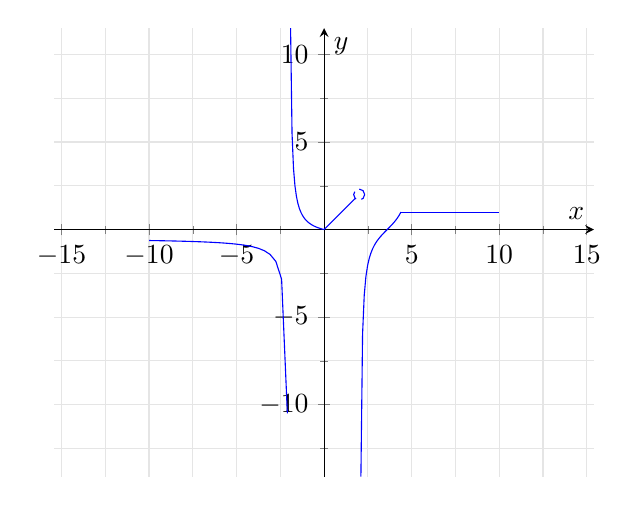
\begin{tikzpicture}
				\begin{axis}[axis lines=middle,xlabel=$x$,ylabel=$y$,axis equal,grid=both,minor tick num=1,grid style={solid, gray!20}]
					\addplot[domain=-10:-2.1,blue] {1/(x+2)-0.5};
					\addplot[domain=-2:0,blue] {1/(x+2)-0.5};
					\addplot[domain=0:2,blue] {x};
					\addplot[domain=2.1:4.386,blue] {tan(deg(x-3.6))};
					\addplot[domain=4.386:10,blue] {1};
					\addplot+[only marks,mark=*,mark options={scale=1, fill=white},text mark as node=true,blue] coordinates {
					    (2,2)};
				\end{axis}
		\end{tikzpicture}
		\end{center}
\setcounter{enumi}{8}
	\item A parking lot charges \$3 for the first hour (or only part of an hour) and \$2 for each succeeding hour (or part), up to a daily maximum of \$10.
	\begin{enumerate}
		\item Sketch the graph of the cost of parking at this lot as a function of the time parked there.
		
			\begin{center}
			\pgfplotsset{compat=1.8,width=0.6\linewidth,height=7cm}
			
 			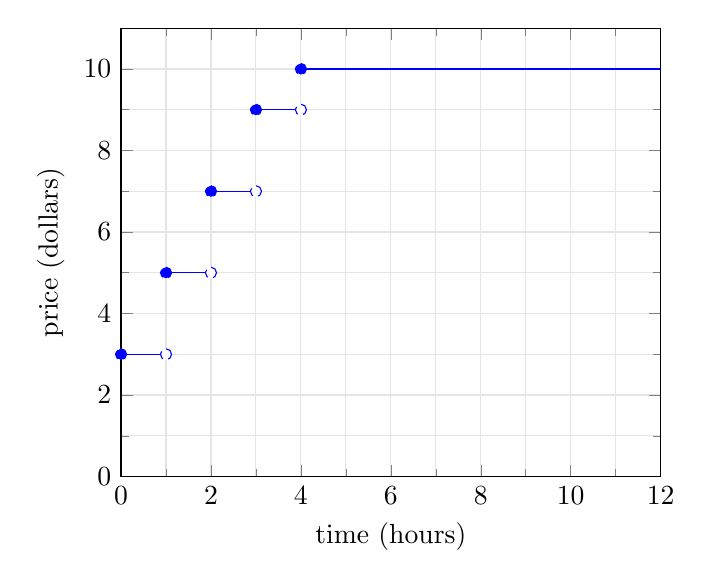
\begin{tikzpicture}
				\begin{axis}[xmin=0,xmax=12,ymin=0,xlabel=time (hours),ylabel=price (dollars),grid=both,minor tick num=1,grid style={solid, gray!20}]
					\addplot[domain=0:1,blue] {3};
					\addplot[domain=1:2,blue] {5};
					\addplot[domain=2:3,blue] {7};
					\addplot[domain=3:4,blue] {9};
					\addplot[domain=4:12,blue] {10};
					\addplot+[only marks,mark=*,mark options={fill=white},text mark as node=false,blue] coordinates {
					    (1,3)
					    (2,5)
					    (3,7)
					    (4,9)};
					\addplot+[only marks,mark=*,mark options={fill=blue},text mark as node=true,blue] coordinates {
					    (0,3)
					    (1,5)
					    (2,7)
					    (3,9)
					    (4,10)};
				\end{axis}
			\end{tikzpicture}
			\end{center}
		
		\item Discuss the discontinuities of this function and their significance to someone who parks in this lot. \\
			The discontinuities of this function are very significant to a person parking in the lot looking to make their money go the furthest possible. This means, it would be most efficient if you want to stay for 4 hours to really only stay for 3:59, because you would save \$2 in the end, just before the function jumps to a higher price.
	\end{enumerate}
\setcounter{enumi}{15}
	\item Explain why the function is discontinuous at the given number $a$. Sketch the graph of the function:
		
		$$f(x)=\begin{cases} 
      		\frac{x^2-x}{x^2-1} & \text{if } x \neq 1 \\
      		1 & \text{if } x = 1
   		\end{cases} \qquad\ \qquad a=1$$
   		
   		\begin{center}
			\pgfplotsset{compat=1.6,width=0.8\linewidth,height=7cm}
			\pgfplotsset{xmin=-10,xmax=10,ymin=-4,ymax=6,soldot/.style={color=blue,only marks,mark=*}}\pgfplotsset{holdot/.style={color=blue,fill=white,only marks,mark=*}}
 			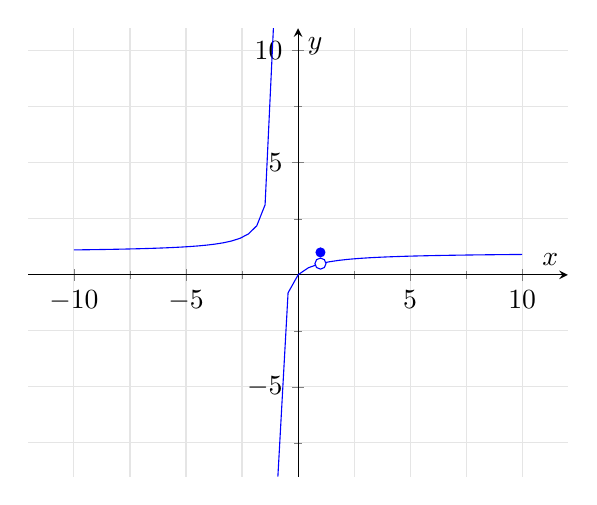
\begin{tikzpicture}
				\begin{axis}[axis lines=middle,xlabel=$x$,ylabel=$y$,axis equal,grid=both,minor tick num=1,grid style={solid, gray!20}]
					\addplot[domain=-10:-1.1,blue] {(x^2-x)/(x^2-1)};
					\addplot[domain=-0.9:10,blue] {(x^2-x)/(x^2-1)};
					\addplot+[only marks,mark=*,mark options={scale=0.8, fill=blue},text mark as node=true,blue] coordinates {
					    (1,1)};
					\addplot+[only marks,mark=*,mark options={scale=1, fill=white},text mark as node=true,blue] coordinates {
					    (1,0.5)};
				\end{axis}
		\end{tikzpicture}
		\end{center}
   		
   		The function is discontinous at number $a$ simply because $a$ is not located along the graph line for the function $\frac{x^2-x}{x^2-1}$. This causes the graph above, with a discontinuity at $x=1$.
   		
\setcounter{enumi}{41}
	\item Use the Intermediate Value Theorem to show that there is a root of the given equation in the specified interval: $\sqrt[\leftroot{-1}\uproot{2}2]{x} =1-x,\quad (0,1)$.
	$$\begin{align}
	\sqrt[\leftroot{-1}\uproot{2}2]{x} &= 1-x \\
	\sqrt[\leftroot{-1}\uproot{2}2]{x} + x -1 &= 0 \\
	\end{align}$$
	$x=0 \\
	\sqrt[\leftroot{-1}\uproot{2}2]{0} + 0 - 1 = -1$
	The curve is below 0!
	
	$x=1 \\
	\sqrt[\leftroot{-1}\uproot{2}2]{1} + 1 -1 = 2 - 1 = 1$
	The curve is above 0!
	
	Because square root is continuous, there is a root to the equation $\sqrt[\leftroot{-1}\uproot{2}2]{x} =1-x$ in the interval $(0,1)$.
\end{enumerate}

\end{document}